\documentclass{exam}
\usepackage{graphicx} % Required for inserting images
\usepackage{amsmath, amsthm, amsfonts, amssymb, amscd, cancel,mathrsfs, mathtools, pinlabel, soul, stmaryrd}


\newcommand{\nbhd}{\ensuremath{\mathcal{N}}}

\newcommand{\N}{\ensuremath{\mathbb{N}}}
\newcommand{\Q}{\ensuremath{\mathbb{Q}}}
\newcommand{\R}{\ensuremath{\mathbb{R}}}
\newcommand{\Z}{\ensuremath{\mathbb{Z}}}
\newcommand{\C}{\ensuremath{\mathbb{C}}}
\renewcommand{\H}{\ensuremath{\mathbb{H}}}
\newcommand{\RP}{\ensuremath{\mathbb{RP}}}
\newcommand{\Sp}{\mathbb{S}}

\renewcommand{\b}{\ensuremath{\mathfrak{b}}}
\newcommand{\SL}{\ensuremath{\mathrm{SL}}}
\newcommand{\PSL}{\ensuremath{\mathrm{PSL}}}


\newcommand{\mobius}{M\"{o}bius }





\title{Spring 2025}
\author{Topological Data Analysis}
\date{Assignment 1}

\begin{document}

\maketitle

\section*{General info} 
\textbf{Deadline:} February 28, 2025 by midnight \\
\textbf{Submission:} Through eLC - Your submission should be a ZIP file containing a PDF file with LaTeX-formatted answers to Part I and a Jupyter Notebook with solutions for Part II.

\section*{Problems}

\subsection*{Part I: Fun with topology and algebraic topology}

\begin{enumerate}
    \item (10 points) Let $f: \Sp^1 \rightarrow \Sp^2$ be a continuous map which is not surjective. Prove that it is homotopic to a constant map.

    \item (10 points) Let $X$ and $Y$ be two homeomorphic topological spaces. Show that if $X$ has dimension $n$, then $Y$ also has dimension $n$.

    \item (10 points) Let $(G,+)$ be a group. Prove that
    $$ \forall g \in G, g+g = 0 \Rightarrow G \hspace{0.2cm} \text{is commutative}.$$

    \item (10 points) Characterize the two surfaces depicted in Figure \ref{fig:surfaces}  in terms of genus, boundary, and orientability.

    \begin{figure}[ht]
        \centering
        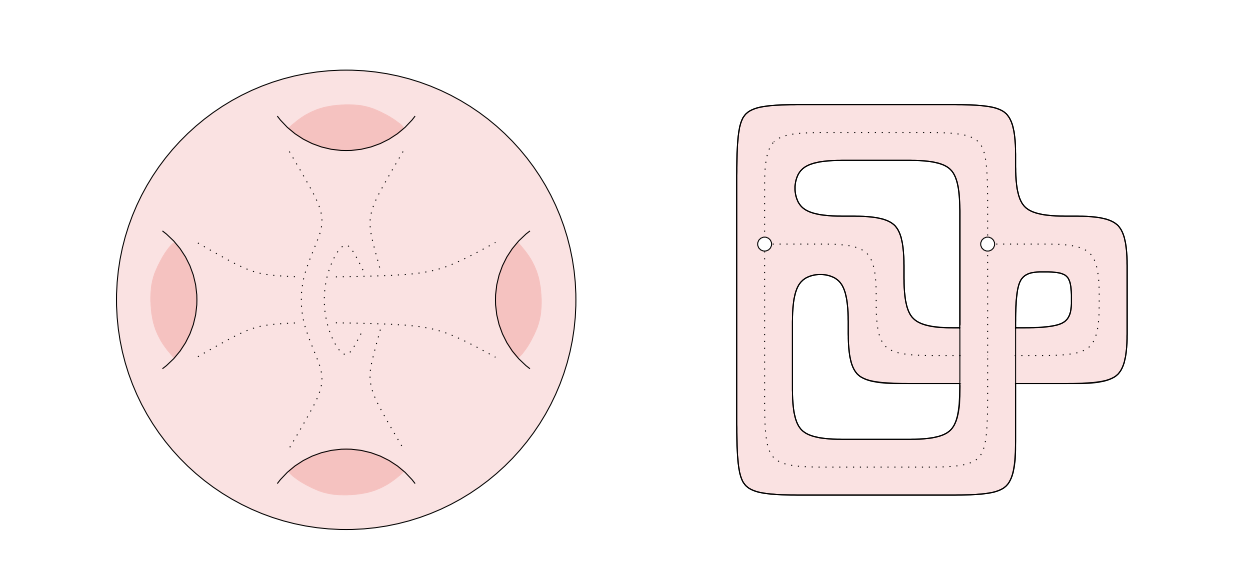
\includegraphics[width=0.5\linewidth]{surfaces.png}
        \caption{Left: a 2-manifold without boundary obtained by adding tunnels inside the sphere. Wee see four tunnel openings and one tunnel passing though a fork of the other. Right: a 2-manifold with boundary obtained by thickening a graph.}
        \label{fig:surfaces}
    \end{figure}

    \item (10 points) Is every graph that can be embedded on the \mobius strip planar?
\end{enumerate}

\newpage

\subsection*{Part II: Fun with python}

\begin{enumerate}
    \item (20 points) Implement the following triangulation of Klein bottle. Then, compute its Euler characteristic and Betti numbers. (You may use gudhi library)

\begin{figure}[ht]
    \centering
    \includegraphics[width=0.3\linewidth]{triangulation_Kleinbottle.png}
    \caption{A triangulation of Klein bottle}
    \label{fig:klein}
\end{figure}


    \item (30 points) Implement the matrix algorithm to decide whether a simplex is positive or negative given a total order and complete the incremental algorithm. Use your final code to compute the Betti numbers of Klein bottle and compare with the answer to the previous question. 
\end{enumerate}


\end{document}
